% Options for packages loaded elsewhere
\PassOptionsToPackage{unicode}{hyperref}
\PassOptionsToPackage{hyphens}{url}
%
\documentclass[
]{book}
\usepackage{lmodern}
\usepackage{amssymb,amsmath}
\usepackage{ifxetex,ifluatex}
\ifnum 0\ifxetex 1\fi\ifluatex 1\fi=0 % if pdftex
  \usepackage[T1]{fontenc}
  \usepackage[utf8]{inputenc}
  \usepackage{textcomp} % provide euro and other symbols
\else % if luatex or xetex
  \usepackage{unicode-math}
  \defaultfontfeatures{Scale=MatchLowercase}
  \defaultfontfeatures[\rmfamily]{Ligatures=TeX,Scale=1}
\fi
% Use upquote if available, for straight quotes in verbatim environments
\IfFileExists{upquote.sty}{\usepackage{upquote}}{}
\IfFileExists{microtype.sty}{% use microtype if available
  \usepackage[]{microtype}
  \UseMicrotypeSet[protrusion]{basicmath} % disable protrusion for tt fonts
}{}
\makeatletter
\@ifundefined{KOMAClassName}{% if non-KOMA class
  \IfFileExists{parskip.sty}{%
    \usepackage{parskip}
  }{% else
    \setlength{\parindent}{0pt}
    \setlength{\parskip}{6pt plus 2pt minus 1pt}}
}{% if KOMA class
  \KOMAoptions{parskip=half}}
\makeatother
\usepackage{xcolor}
\IfFileExists{xurl.sty}{\usepackage{xurl}}{} % add URL line breaks if available
\IfFileExists{bookmark.sty}{\usepackage{bookmark}}{\usepackage{hyperref}}
\hypersetup{
  pdftitle={Knowledge Pool},
  pdfauthor={Institute for Transport Studies (IVe), University of Natural Resources and Life in Vienna},
  hidelinks,
  pdfcreator={LaTeX via pandoc}}
\urlstyle{same} % disable monospaced font for URLs
\usepackage{longtable,booktabs}
% Correct order of tables after \paragraph or \subparagraph
\usepackage{etoolbox}
\makeatletter
\patchcmd\longtable{\par}{\if@noskipsec\mbox{}\fi\par}{}{}
\makeatother
% Allow footnotes in longtable head/foot
\IfFileExists{footnotehyper.sty}{\usepackage{footnotehyper}}{\usepackage{footnote}}
\makesavenoteenv{longtable}
\usepackage{graphicx,grffile}
\makeatletter
\def\maxwidth{\ifdim\Gin@nat@width>\linewidth\linewidth\else\Gin@nat@width\fi}
\def\maxheight{\ifdim\Gin@nat@height>\textheight\textheight\else\Gin@nat@height\fi}
\makeatother
% Scale images if necessary, so that they will not overflow the page
% margins by default, and it is still possible to overwrite the defaults
% using explicit options in \includegraphics[width, height, ...]{}
\setkeys{Gin}{width=\maxwidth,height=\maxheight,keepaspectratio}
% Set default figure placement to htbp
\makeatletter
\def\fps@figure{htbp}
\makeatother
\setlength{\emergencystretch}{3em} % prevent overfull lines
\providecommand{\tightlist}{%
  \setlength{\itemsep}{0pt}\setlength{\parskip}{0pt}}
\setcounter{secnumdepth}{5}
\usepackage{booktabs}
\usepackage{amsthm}
\makeatletter
\def\thm@space@setup{%
  \thm@preskip=8pt plus 2pt minus 4pt
  \thm@postskip=\thm@preskip
}
\makeatother
\usepackage[]{natbib}
\bibliographystyle{apalike}

\title{Knowledge Pool}
\author{Institute for Transport Studies (IVe), University of Natural Resources and Life in Vienna}
\date{2021-01-18}

\begin{document}
\maketitle

{
\setcounter{tocdepth}{1}
\tableofcontents
}
\hypertarget{preface}{%
\chapter*{Preface}\label{preface}}
\addcontentsline{toc}{chapter}{Preface}

This is a \emph{continuously developing} database, which is a part of \href{https://www.davemos.online/}{DAVeMOS} project. It aims at gathering concepts and evidence of the systemic impact of transport digitalisation and automation. Therefore, the authors of this work welcome any feedback on changes and suggestions for additional content that the readers may have.

For further inputs please contact the corresponding author \emph{Martyna Bogacz} on the following email address: xxx

The knowledge pool was last compiled on:

\begin{verbatim}
## [1] "18 January 2021"
\end{verbatim}

\hypertarget{table-of-content}{%
\chapter*{Table of content}\label{table-of-content}}
\addcontentsline{toc}{chapter}{Table of content}

\begin{enumerate}
\def\labelenumi{\arabic{enumi}.}
\tightlist
\item
  Introduction to the knowledge pool \ref{intro}
\item
  Physical road infrastructure \ref{infrastructure}
\item
  Highway infrastructure management \ref{highway}
\item
  Traffic management \ref{traffic}
\item
  Road pricing \ref{pricing}
\item
  Digital road infrastructure and connectivity \ref{digital}
\item
  Passenger information system \ref{passenger}
\item
  Multimodal integrated system \ref{multimodal}
\item
  Connected and autonomous driving \ref{connected}
\item
  On-board technology for connected and automated vehicles \ref{onboard}
\item
  Freight and commercial transport \ref{freight}
\item
  Collective mobility vehicles \ref{collective}
\item
  Big data \ref{big}
\item
  Shared mobility \ref{shared}
\item
  Alternative power sources \ref{alternative}
\end{enumerate}

\hypertarget{intro}{%
\chapter{Introduction}\label{intro}}

This work gathers and defines essential concepts related to automation and digitalisation of transport system together with the description of their impact, both negative and positive on \textbf{individual}, \textbf{systemic} and \textbf{economy level}. This knowledge pool is driven by the fact that automation and digitalisation are progressing quickly, although not uniformly across all areas within transport context. Therefore, to understand spectrum of possibilities that they bring, it is necessary to explain key concepts, demonstrate their level of maturity and current market penetration, and finally assess their impact on different levels. Given this approach, the page of each topic contains the following elements:\textbf{definition} of the phenomenon,
\textbf{key stakeholders} who are the main parties responsible for and affected by the given technological development. Then, we include two subsections on \textbf{current state of art in research and practice}. The former one summarizes the most recent research in a given topic while the latter explains the current stage of implementation of given technology in the real world. Further, section named \textbf{relevant initatives in Austria} covers the leading initaitives within given topic and potential for Austrain actors. Moreover, we provide the summary table of the impacts of the concept on selected \textbf{sustainable development goals} (SDGs). Beyond, to provide an objective measure of technology maturity within each topic we include so-called \textbf{technology readiness scale} (Willismson \& Beasley, 2011) and \textbf{societal readiness scale}, as described below:

\begin{figure}
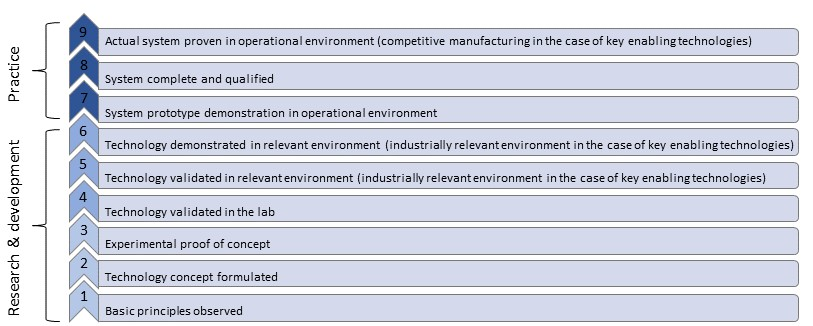
\includegraphics[width=2\linewidth]{image/TRL} \caption{Technology readiness scale}\label{fig:unnamed-chunk-2}
\end{figure}

\begin{figure}
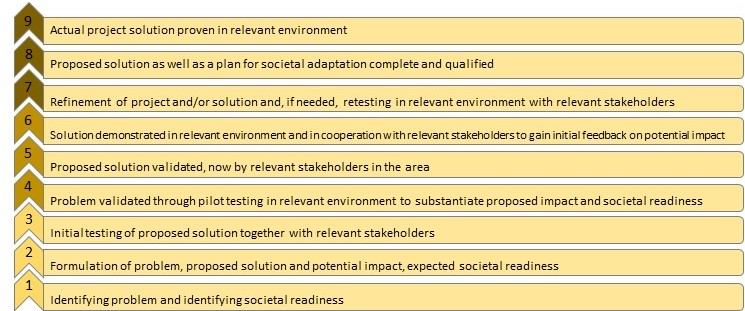
\includegraphics[width=2\linewidth]{image/SRL} \caption{Societal readiness scale}\label{fig:unnamed-chunk-3}
\end{figure}

Finally, we provide a list of \textbf{outstanding questions} and \textbf{links to additional sources} on the topic.

\textbf{References}

\begin{itemize}
\tightlist
\item
  Williamson, R., \& Beasley, J. (2011). Automotive technology and manufacturing readiness levels: a guide to recognised stages of development within the automotive industry. URN11/672.
\end{itemize}

\hypertarget{infrastructure}{%
\chapter{Physical road infrastructure}\label{infrastructure}}

\hypertarget{dedicated-lanes-for-connected-and-automated-vehicles-cav}{%
\section{Dedicated lanes for connected and automated vehicles (CAV)}\label{dedicated-lanes-for-connected-and-automated-vehicles-cav}}

\hypertarget{synonyms}{%
\subsection*{Synonyms}\label{synonyms}}
\addcontentsline{toc}{subsection}{Synonyms}

\emph{AV-dedicated lanes}, \emph{dedicated corridors}

\hypertarget{definition}{%
\subsection*{Definition}\label{definition}}
\addcontentsline{toc}{subsection}{Definition}

Dedicated lane for connected and autonomous vehicles features additional infrastructure or sensors to increase the reliability of Advanced Driver Assistant Systems (ADAS). Only automated driving vehicles are allowed to drive on these lanes. The typical applications include cooperative and adaptive cruise control based on sensors with the infrastructure, lane keeping, fuel use optimization and road pricing possibilities (Broek et al., 2011). The introduction of dedicated lanes for CAV is expected to have direct consequences on the traffic flow on the highways and a nearby road network. In particular, a study conducted in Singapore showed that dedicated lanes on the highways can reduce travel time of CAVs by approximately 25\% (if the saturation on the lane is not reached) at the cost of a delay for conventional cars of approximately 7\%, due to the reduced capacity (Ivanchev et al., 2017). They were also demonstrated to have a positive effect on fuel consumption.
Moreover, the throughput, defined as a number of vehicles passing through the road in a given time interval, increased as a result of introduction of dedicated lanes for AVs (Kumar et al., 2020). This effect, however, was associated with a decrease in throughput of smaller roads due to the preference of AVs for highways because of time savings, which in turn can result in time loss for conventional cars. What is more, the benefits from increased capacity of AV-only lanes can be further amplified through setting a higher speed limits for these lanes (Ye \& Yamamoto, 2018). With respect to the demand for different road types the study found that the introduction of dedicated CAV lanes will increase the demand of conventional cars for major road (but smaller than highways) and minor roads as a substitution for more congested highways due to the dedicated AV lanes.
In contrast, study by Chen et al.~(2016) showed that the implementation of CAV dedicated lanes has a potential of maximizing traffic capacity on these lanes in a mix-traffic context while having effectively no impact on conventional traffic capacity. Further, in order to use efficiently CAV dedicated lanes, which may be underutilized at the early stage, it is proposed to allow conventional cars to enter the AVs-only lanes after toll payment. This solution stems from currently operational across the world High Occupancy Vehicle (HOV) lanes. This joint approach is claimed to improve the throughput of individual road as well as enhance system-wide flow distribution within the network (Liu \& Song, 2019).

\hypertarget{key-stakeholders}{%
\subsection*{Key stakeholders}\label{key-stakeholders}}
\addcontentsline{toc}{subsection}{Key stakeholders}

\begin{itemize}
\tightlist
\item
  \textbf{Affected}: Conventional Cars' Drivers, Car Manufacturers, Insurers
\item
  \textbf{Responsible}: Road Infrastructure Agencies, Local and National Governments
\end{itemize}

\hypertarget{current-state-of-art-in-research}{%
\subsection*{Current state of art in research}\label{current-state-of-art-in-research}}
\addcontentsline{toc}{subsection}{Current state of art in research}

Current research focuses on gathering the evidence of the impact of the introduction of dedicated lanes on traffic flow, driver behavior adoption, safety and efficiency. Furthermore, it analyses the factors which influence them, by testing different design and operation configurations, road types and utilization policies (Rad et al., 2020). Both, field operational testing and driving simulator studies have been conducted to investigate the influence of different designs of dedicated lanes on drivers in conventional cars and those featuring some degree of automation (Guin et al., 2008, Zhong, 2018). In particular, a number of studies compared distinct access types of dedicated lanes (Zhong, 2018, Yang et al., 2019). They showed that dedicated lanes with limited access performed better in terms of travel time and throughput compared to dedicated lanes with continuous access. Moreover, the probability of vehicles platooning was significantly higher on dedicated lanes with limited access. On the other hand, it was showed that collision rates near the entry or exit of these limited access lanes are higher (Rad et al.~2020).

\hypertarget{current-state-of-art-in-practice}{%
\subsection*{Current state of art in practice}\label{current-state-of-art-in-practice}}
\addcontentsline{toc}{subsection}{Current state of art in practice}

Currently state of Michigan together with several private partners including Ford and Alphabet Inc.~are planning to dedicate 65 km of a highway between Detroit and Ann Arbor for the sole movement of autonomous vehicles including buses and shuttles (Krisher \& Eggert, 2020). Similar initiatives are taking place in other countries, for instance, China set out to build nearly 100 km of 8-lane highway linking Beijing and the Xiongan New Area, from which 2 lanes will be allocated for the automated traffic. The completion of the construction phase is predicted by the end of 2020, while its opening is for traffic is expected in June 2021 (Syncedreview.com, 2020). In Europe, there is on-going SHOW (SHared automation Operating models for Worldwide adoption) project which aims to deploy about seventy automated vehicles in 21 European cities. To assess how they can best be integrated vehicles will be used in different settings in mixed traffic and dedicated lanes. However, for safety reasons the driver will be on-board (CORDIS, 2020).

\hypertarget{relevant-initiatives-in-austria}{%
\subsection*{Relevant initiatives in Austria}\label{relevant-initiatives-in-austria}}
\addcontentsline{toc}{subsection}{Relevant initiatives in Austria}

\begin{itemize}
\tightlist
\item
  \href{https://www.tugraz.at/fileadmin/user_upload/Institute/IHF/Projekte/ENABLE-S3_SummaryofResults_May2019.pdf}{tugraz.at}
\item
  \href{https://www.ait.ac.at/themen/verkehrssicherheit-und-unfallforschung/projects/via-autonom/}{ait.ac.at}
\end{itemize}

\hypertarget{impacts-with-respect-to-sustainable-development-goals-sdgs}{%
\subsection*{Impacts with respect to Sustainable Development Goals (SDGs)}\label{impacts-with-respect-to-sustainable-development-goals-sdgs}}
\addcontentsline{toc}{subsection}{Impacts with respect to Sustainable Development Goals (SDGs)}

\begin{longtable}[]{@{}ccccc@{}}
\toprule
\begin{minipage}[b]{0.17\columnwidth}\centering
Impact level\strut
\end{minipage} & \begin{minipage}[b]{0.16\columnwidth}\centering
Indicator\strut
\end{minipage} & \begin{minipage}[b]{0.17\columnwidth}\centering
Impact direction\strut
\end{minipage} & \begin{minipage}[b]{0.17\columnwidth}\centering
Goal description and number\strut
\end{minipage} & \begin{minipage}[b]{0.17\columnwidth}\centering
Source\strut
\end{minipage}\tabularnewline
\midrule
\endhead
\begin{minipage}[t]{0.17\columnwidth}\centering
Individual\strut
\end{minipage} & \begin{minipage}[t]{0.16\columnwidth}\centering
Fuel consumption reduced\strut
\end{minipage} & \begin{minipage}[t]{0.17\columnwidth}\centering
\textbf{+}\strut
\end{minipage} & \begin{minipage}[t]{0.17\columnwidth}\centering
Environmental sustainability (\emph{7,12-13,15})\strut
\end{minipage} & \begin{minipage}[t]{0.17\columnwidth}\centering
Ivanchev et al., 2017\strut
\end{minipage}\tabularnewline
\begin{minipage}[t]{0.17\columnwidth}\centering
Individual\strut
\end{minipage} & \begin{minipage}[t]{0.16\columnwidth}\centering
Travel time reduced\strut
\end{minipage} & \begin{minipage}[t]{0.17\columnwidth}\centering
\textbf{+}\strut
\end{minipage} & \begin{minipage}[t]{0.17\columnwidth}\centering
Sustainable economic development (\emph{8,11})\strut
\end{minipage} & \begin{minipage}[t]{0.17\columnwidth}\centering
Zhong, 2018;Yang et al., 2019\strut
\end{minipage}\tabularnewline
\begin{minipage}[t]{0.17\columnwidth}\centering
Systemic\strut
\end{minipage} & \begin{minipage}[t]{0.16\columnwidth}\centering
Collision rate reduced\strut
\end{minipage} & \begin{minipage}[t]{0.17\columnwidth}\centering
\textbf{+}\strut
\end{minipage} & \begin{minipage}[t]{0.17\columnwidth}\centering
Health \& Wellbeing (\emph{3})\strut
\end{minipage} & \begin{minipage}[t]{0.17\columnwidth}\centering
Zhang et al., 2020\strut
\end{minipage}\tabularnewline
\begin{minipage}[t]{0.17\columnwidth}\centering
Systemic\strut
\end{minipage} & \begin{minipage}[t]{0.16\columnwidth}\centering
Emissions rate reduced\strut
\end{minipage} & \begin{minipage}[t]{0.17\columnwidth}\centering
\textbf{+}\strut
\end{minipage} & \begin{minipage}[t]{0.17\columnwidth}\centering
Environmental sustainability (\emph{7,12-13,15})\strut
\end{minipage} & \begin{minipage}[t]{0.17\columnwidth}\centering
Al Alam at al., 2010\strut
\end{minipage}\tabularnewline
\begin{minipage}[t]{0.17\columnwidth}\centering
Systemic\strut
\end{minipage} & \begin{minipage}[t]{0.16\columnwidth}\centering
Congestion\strut
\end{minipage} & \begin{minipage}[t]{0.17\columnwidth}\centering
\textbf{\textasciitilde{}}\strut
\end{minipage} & \begin{minipage}[t]{0.17\columnwidth}\centering
Sustainable economic development (\emph{8,11})\strut
\end{minipage} & \begin{minipage}[t]{0.17\columnwidth}\centering
Ivanchev et al., 2017;Kumar et al., 2020\strut
\end{minipage}\tabularnewline
\begin{minipage}[t]{0.17\columnwidth}\centering
Systemic\strut
\end{minipage} & \begin{minipage}[t]{0.16\columnwidth}\centering
Novel designs tested\strut
\end{minipage} & \begin{minipage}[t]{0.17\columnwidth}\centering
\textbf{+}\strut
\end{minipage} & \begin{minipage}[t]{0.17\columnwidth}\centering
Innovation \& Infrastructure (\emph{9})\strut
\end{minipage} & \begin{minipage}[t]{0.17\columnwidth}\centering
Guin et al., 2008;Zhong, 2018;Krisher \& Eggert, 2020\strut
\end{minipage}\tabularnewline
\begin{minipage}[t]{0.17\columnwidth}\centering
Systemic\strut
\end{minipage} & \begin{minipage}[t]{0.16\columnwidth}\centering
SHOW EU initiative\strut
\end{minipage} & \begin{minipage}[t]{0.17\columnwidth}\centering
\textbf{+}\strut
\end{minipage} & \begin{minipage}[t]{0.17\columnwidth}\centering
Partnership \& collaborations (\emph{17})\strut
\end{minipage} & \begin{minipage}[t]{0.17\columnwidth}\centering
CORDIS, 2020\strut
\end{minipage}\tabularnewline
\bottomrule
\end{longtable}

\hypertarget{technology-and-societal-readiness-level}{%
\subsection*{Technology and societal readiness level}\label{technology-and-societal-readiness-level}}
\addcontentsline{toc}{subsection}{Technology and societal readiness level}

\begin{longtable}[]{@{}cc@{}}
\toprule
TRL & SRL\tabularnewline
\midrule
\endhead
5-6 & 1-3\tabularnewline
\bottomrule
\end{longtable}

\hypertarget{open-questions}{%
\subsection*{Open questions}\label{open-questions}}
\addcontentsline{toc}{subsection}{Open questions}

\begin{enumerate}
\def\labelenumi{\arabic{enumi}.}
\tightlist
\item
  What are the potential benefits of dedicated AV lanes when coupled with smart platooning strategies?
\item
  How and to what degree will joint concepts by automotive sector, fleet and road
  operators will improve traffic management establishing dynamic traffic regulations even across
  borders?
\item
  What are the roles and responsibilities of the different stakeholders of physical infrastructure for connected and automated vehicles?
\item
  Should the vehicle cope with any road infrastructure, and if not, what demands can be set to adapt the existing infrastructure?
\item
  How to ensure continuity between those different environments?
\item
  Which tools (e.g.~micro- and macroscopic transport modelling, impact assessment) can enable
  cities to assess the impact of automated vehicles on their physical road infrastructure and
  balance the needs of automated vehicles against the needs of existing modes (conventional
  vehicles, public transport, pedestrians and cyclists). (ERTRAC, 2019)
\end{enumerate}

\hypertarget{further-links}{%
\subsection*{Further links}\label{further-links}}
\addcontentsline{toc}{subsection}{Further links}

\begin{itemize}
\tightlist
\item
  \href{https://knowledge-base.connectedautomateddriving.eu/wp-content/uploads/2019/12/SMART_2010-0064-study-report-final_V1-2.pdf}{knowledge base}
\item
  \href{https://show-project.eu/}{show project}
\end{itemize}

\hypertarget{references}{%
\subsection*{References}\label{references}}
\addcontentsline{toc}{subsection}{References}

\begin{itemize}
\tightlist
\item
  Al Alam, A., Gattami, A., \& Johansson, K. H. (2010, September). An experimental study on the fuel reduction potential of heavy duty vehicle platooning. In 13th International IEEE Conference on Intelligent Transportation Systems (pp.~306-311). IEEE.
  Broek, S. M., van Nunen, E., \& Zwijnenberg, H. (2011). Definition of necessary vehicle and infrastructure systems for automated driving. Retrieved January, 3, 2017.
\item
  Chen, Z., He, F., Zhang, L., \& Yin, Y. (2016). Optimal deployment of autonomous vehicle lanes with endogenous market penetration. Transportation Research Part C: Emerging Technologies, 72, 143-156.
\item
  CORDIS \textbar{} European Commission. (20 Apr 2020). Retrieved 13 November 2020, from \url{https://cordis.europa.eu/project/id/875530}
\item
  ERTRAC Working Group. (2019). Connected Automated Driving Roadmap. version, 8, 2019-08.
\item
  Guin, A., Hunter, M., \& Guensler, R. (2008). Analysis of reduction in effective capacities of high-occupancy vehicle lanes related to traffic behavior. Transportation Research Record, 2065(1), 47-53.
\item
  Ivanchev, J., Knoll, A., Zehe, D., Nair, S., \& Eckhoff, D. (2017). Potentials and implications of dedicated highway lanes for autonomous vehicles. arXiv preprint arXiv:1709.07658.
\item
  Krisher, T., \& Eggert, D. (14 Aug 2020). Michigan plans dedicated road lanes for autonomous vehicles. Retrieved 12 November 2020, from \url{https://abcnews.go.com/Technology/wireStory/michigan-plans-dedicated-road-lanes-autonomous-vehicles-72352758}
\item
  Kumar, A., Guhathakurta, S., \& Venkatachalam, S. (2020). When and where should there be dedicated lanes under mixed traffic of automated and human-driven vehicles for system-level benefits?. Research in Transportation Business \& Management, 100527.
\item
  Liu, Z., \& Song, Z. (2019). Strategic planning of dedicated autonomous vehicle lanes and autonomous vehicle/toll lanes in transportation networks. Transportation Research Part C: Emerging Technologies, 106, 381-403.
\item
  Rad, S. R., Farah, H., Taale, H., van Arem, B., \& Hoogendoorn, S. P. (2020). Design and operation of dedicated lanes for connected and automated vehicles on motorways: A conceptual framework and research agenda. Transportation Research Part C: Emerging Technologies, 117, 102664.
\item
  Syncedreview.com (31 Aug 2020). Beijing Builds 100km Highway Lanes for Self-Driving Cars with Unmanned Machineries. Retrieved 12 November 2020, from \url{https://syncedreview.com/2020/08/31/beijing-builds-100km-highway-lanes-for-self-driving-cars-with-unmanned-machineries/}
\item
  Yang, D., Farah, H., Schoenmakers, M. J., \& Alkim, T. (2019). Human drivers behavioural adaptation when driving next to a platoon of automated vehicles on a dedicated lane and implications on traffic flow: a driving simulator and microscopic simulation study in the Netherlands. In 98th Annual Meeting of the Transportation Research Board (pp.~19-00582).
\item
  Ye, L., \& Yamamoto, T. (2018). Impact of dedicated lanes for connected and autonomous vehicle on traffic flow throughput. Physica A: Statistical Mechanics and its Applications, 512, 588-597.
\item
  Zhang, J., Wu, K., Cheng, M., Yang, M., Cheng, Y., \& Li, S. (2020). Safety Evaluation for Connected and Autonomous Vehicles' Exclusive Lanes considering Penetrate Ratios and Impact of Trucks Using Surrogate Safety Measures. Journal of advanced transportation, 2020.
\item
  Zhong, Z. (2018). Assessing the effectiveness of managed lane strategies for the rapid deployment of cooperative adaptive cruise control technology.
\end{itemize}

\hypertarget{cooperative-lane-control-for-connected-and-automated-vehicles}{%
\section{Cooperative lane control for connected and automated vehicles}\label{cooperative-lane-control-for-connected-and-automated-vehicles}}

\hypertarget{operational-design-domains}{%
\section{Operational design domains}\label{operational-design-domains}}

\hypertarget{rail-crossing-information-system}{%
\section{Rail crossing information system}\label{rail-crossing-information-system}}

\hypertarget{electric-road-system}{%
\section{Electric road system}\label{electric-road-system}}

\hypertarget{high-occupancy-toll-lanes}{%
\section{High occupancy toll lanes}\label{high-occupancy-toll-lanes}}

\hypertarget{public-transport-priority-systems}{%
\section{Public transport priority systems}\label{public-transport-priority-systems}}

\hypertarget{transformation-of-public-space-and-digital-solutions}{%
\section{Transformation of public space and digital solutions}\label{transformation-of-public-space-and-digital-solutions}}

\hypertarget{highway}{%
\chapter{Highway infrastructure management}\label{highway}}

\hypertarget{unmanned-aerial-vehicles-for-infrastructure-mainteinance}{%
\section{Unmanned aerial vehicles for infrastructure mainteinance}\label{unmanned-aerial-vehicles-for-infrastructure-mainteinance}}

\hypertarget{synonyms-1}{%
\subsection*{Synonyms}\label{synonyms-1}}
\addcontentsline{toc}{subsection}{Synonyms}

\emph{Drones, remotely piloted vehicles, remotely piloted aircraft, uav}

\hypertarget{definition-1}{%
\subsection*{Definition}\label{definition-1}}
\addcontentsline{toc}{subsection}{Definition}

Unmanned Aerial Vehicles (UAVs), commonly known as drones are promising technologies that can be used in inspection and data gathering for infrastructure maintenance and management purposes. These include, for example, detection of wear and tear, monitoring of the progress at a highway construction site or the analysis of traffic (Frederiksen et al., 2019). UAVs typically include a portable control station for the human operator and under current legislation their operation in urban areas is limited to flying within visual line of sight (VLOS). UAVs typically feature various sensors and recorders, including video, far and near infrared, radar or laser-based range finders and specialized communication devices (Shaghlil \& Khalafallah, 2018). Majority of them can transfer real-time data between the UAV and the control station. Moreover, some feature additional onboard data storage capabilities for enhanced data collection (Shaghlil \& Khalafallah, 2018). The use of drones for infrastructure-related tasks provide not only savings with respect to time, labor and costs, but they also allow for reduction in risks when dangerous operations usually performed by human can be substituted with drones. Finally, the environmental impact is diminished when drones, which produce considerably less CO2, are used instead of currently employed helicopters. Nevertheless, the use of drones as a tool for inspecting infrastructure can also pose certain challenges with respect to current technology, legal framework, privacy concerns and social acceptance.

\hypertarget{key-stakeholders-1}{%
\subsection*{Key stakeholders}\label{key-stakeholders-1}}
\addcontentsline{toc}{subsection}{Key stakeholders}

\begin{itemize}
\tightlist
\item
  \textbf{Affected}: Direct users of the roads and beneficiaries affected by the supply of transport services
\item
  \textbf{Responsible}: Government agencies responsible for planning, executing, and financing of maintenance activities, citizens, contractors and subcontractors, private companies and manufacturers
\end{itemize}

\hypertarget{current-state-of-art-in-research-1}{%
\subsection*{Current state of art in research}\label{current-state-of-art-in-research-1}}
\addcontentsline{toc}{subsection}{Current state of art in research}

Current research efforts and field trials-based studies are advocating the case of using UAVs for bridge inspection and monitoring. Previous study presented a proof of concept of utilising UAVs for bridge and high mast luminaires. Several experiments in controlled conditions were performed to test UAV response in relation to wind conditions. Moreover, image quality was examined in different flight scenarios, low light conditions, altitude and payload (Otero et al., 2015). Overall, the results are in favour of using drones for infrastructure inspections, not just in terms of saving human labor but also detecting the damages. The advantages of the drone use were also demonstrated in terms of reduced traffic control and decreased use of under bridge inspection vehicles (Zink and Lovelace, 2015). On the other hand, specific skills of the drone operators were found to hinder efficient use of drones for large-scale bridges (Wu et al., 2018). Further, some technological barriers also slow down the popularity of drones in infrastructure inspection, where an average flight time of the drone given its battery life is approximately 30 minutes. Therefore, current research aims at increasing the energy-efficiency by the use of path planning and algorithms to minimize energy utilization while maximizing coverage for traffic monitoring (Outay et al., 2020).

\hypertarget{current-state-of-art-in-practice-1}{%
\subsection*{Current state of art in practice}\label{current-state-of-art-in-practice-1}}
\addcontentsline{toc}{subsection}{Current state of art in practice}

Current use of drones is heavily regulated by national and international governments worldwide where the most considerable restriction is the requirement for drones to remain under VLOS of the controller. Beyond, the regulatory bodies put forward various specification with respect to physical aspects of the drones such as weight or sensors, training requirement of the operators and drones', data acquisition regulations and operation itself such as flight timeframe, altitude etc. (FAA, 2016; Outay at al., 2020). All of them, significantly restrict fast and wide application of drones in different areas. Therefore, the authorities attempt to provide regulations to tackle safety and privacy as well as noise concerns of the citizens. At the moment drones are used in oil and gas industry to conduct local surveys in off-shore facilities (Undertaking, 2016). Meanwhile in the transport sector, Danish company Dronops, after safety clearance, has been granted permission from Danish Road Authority to fly along a highway to monitor the traffic, where drone provides data from multiple sensors as well as video recordings. At the moment, the drone can only fly in good weather conditions and it is cable-linked to its power source located on the ground to allow for continuous day-long monitoring at 120 m above the ground. Importantly, the output data is used by Danish Road Authority and local council (Frederiksen et al., 2019).

\hypertarget{relevant-initiatives-in-austria-1}{%
\subsection*{Relevant initiatives in Austria}\label{relevant-initiatives-in-austria-1}}
\addcontentsline{toc}{subsection}{Relevant initiatives in Austria}

\begin{itemize}
\tightlist
\item
  \href{https://smartcity.wien.gv.at/site/en/smart-inspection/}{smartcity.wien}
\end{itemize}

\hypertarget{impacts-with-respect-to-sustainable-development-goals-sdgs-1}{%
\subsection*{Impacts with respect to Sustainable Development Goals (SDGs)}\label{impacts-with-respect-to-sustainable-development-goals-sdgs-1}}
\addcontentsline{toc}{subsection}{Impacts with respect to Sustainable Development Goals (SDGs)}

\begin{longtable}[]{@{}ccccc@{}}
\toprule
\begin{minipage}[b]{0.17\columnwidth}\centering
Impact level\strut
\end{minipage} & \begin{minipage}[b]{0.16\columnwidth}\centering
Indicator\strut
\end{minipage} & \begin{minipage}[b]{0.17\columnwidth}\centering
Impact direction\strut
\end{minipage} & \begin{minipage}[b]{0.17\columnwidth}\centering
Goal description and number\strut
\end{minipage} & \begin{minipage}[b]{0.17\columnwidth}\centering
Source\strut
\end{minipage}\tabularnewline
\midrule
\endhead
\begin{minipage}[t]{0.17\columnwidth}\centering
Individual\strut
\end{minipage} & \begin{minipage}[t]{0.16\columnwidth}\centering
Employees risk reduced\strut
\end{minipage} & \begin{minipage}[t]{0.17\columnwidth}\centering
\textbf{+}\strut
\end{minipage} & \begin{minipage}[t]{0.17\columnwidth}\centering
Health \& Wellbeing (\emph{3})\strut
\end{minipage} & \begin{minipage}[t]{0.17\columnwidth}\centering
Outay et al., 2020\strut
\end{minipage}\tabularnewline
\begin{minipage}[t]{0.17\columnwidth}\centering
Systemic\strut
\end{minipage} & \begin{minipage}[t]{0.16\columnwidth}\centering
Road safety increased\strut
\end{minipage} & \begin{minipage}[t]{0.17\columnwidth}\centering
\textbf{+}\strut
\end{minipage} & \begin{minipage}[t]{0.17\columnwidth}\centering
Health \& Wellbeing (\emph{3})\strut
\end{minipage} & \begin{minipage}[t]{0.17\columnwidth}\centering
Outay et al., 2020\strut
\end{minipage}\tabularnewline
\begin{minipage}[t]{0.17\columnwidth}\centering
Systemic\strut
\end{minipage} & \begin{minipage}[t]{0.16\columnwidth}\centering
Emissions rate reduced\strut
\end{minipage} & \begin{minipage}[t]{0.17\columnwidth}\centering
\textbf{+}\strut
\end{minipage} & \begin{minipage}[t]{0.17\columnwidth}\centering
Environmental sustainability (\emph{7,12-13,15})\strut
\end{minipage} & \begin{minipage}[t]{0.17\columnwidth}\centering
Outay et al., 2020\strut
\end{minipage}\tabularnewline
\begin{minipage}[t]{0.17\columnwidth}\centering
Systemic\strut
\end{minipage} & \begin{minipage}[t]{0.16\columnwidth}\centering
Job posts created\strut
\end{minipage} & \begin{minipage}[t]{0.17\columnwidth}\centering
\textbf{+}\strut
\end{minipage} & \begin{minipage}[t]{0.17\columnwidth}\centering
Sustainable economic development (\emph{8,11})\strut
\end{minipage} & \begin{minipage}[t]{0.17\columnwidth}\centering
Jenkins \& Vasigh, 2013\strut
\end{minipage}\tabularnewline
\begin{minipage}[t]{0.17\columnwidth}\centering
Systemic\strut
\end{minipage} & \begin{minipage}[t]{0.16\columnwidth}\centering
Faster road infrastructure innovation\strut
\end{minipage} & \begin{minipage}[t]{0.17\columnwidth}\centering
\textbf{+}\strut
\end{minipage} & \begin{minipage}[t]{0.17\columnwidth}\centering
Innovation \& Infrastructure (9)\strut
\end{minipage} & \begin{minipage}[t]{0.17\columnwidth}\centering
Fan \& Saadeghvaziri, 2019\strut
\end{minipage}\tabularnewline
\bottomrule
\end{longtable}

\hypertarget{technology-and-societal-readiness-level-1}{%
\subsection*{Technology and societal readiness level}\label{technology-and-societal-readiness-level-1}}
\addcontentsline{toc}{subsection}{Technology and societal readiness level}

\begin{longtable}[]{@{}cc@{}}
\toprule
TRL & SRL\tabularnewline
\midrule
\endhead
3-4 & 5-7\tabularnewline
\bottomrule
\end{longtable}

\hypertarget{open-questions-1}{%
\subsection*{Open questions}\label{open-questions-1}}
\addcontentsline{toc}{subsection}{Open questions}

\begin{enumerate}
\def\labelenumi{\arabic{enumi}.}
\tightlist
\item
  What are the factors influencing social acceptability of drones?
\item
  What actions from the policymakers need to be undertaken to minimalize cyber-attacks?
\item
  What aspects need to be considered by the governments before the integration of more sensors to record other relevant data along with the integration of video data with other geospatial information?
\end{enumerate}

\hypertarget{further-links-1}{%
\subsection*{Further links}\label{further-links-1}}
\addcontentsline{toc}{subsection}{Further links}

\begin{itemize}
\tightlist
\item
  \href{https://www.rolandberger.com/en/Insights/Publications/Drones-The-future-of-asset-inspection.html}{rolandberger}
\end{itemize}

\hypertarget{references-1}{%
\subsection*{References}\label{references-1}}
\addcontentsline{toc}{subsection}{References}

\begin{itemize}
\tightlist
\item
  FAA News, 2016, Summary of Small Unmanned Aircraft Rule (Part 107), Federal Aviation Authority, Washington DC, 20591, Accessed on May 2020, \url{https://www.faa.gov/uas/media/Part_107_Summary.pdf}.
\item
  Fan, J., \& Saadeghvaziri, M. A. (2019). Applications of Drones in Infrastructures: Challenges and Opportunities. International Journal of Mechanical and Mechatronics Engineering, 13(10), 649-655.
\item
  Frederiksen, M. H., Mouridsen, O. A. V., \& Knudsen, M. P. (2019). Drones for inspection of infrastructure: Barriers, opportunities and successful uses.
\item
  Jenkins, D., \& Vasigh, B. (2013). The economic impact of unmanned aircraft systems integration in the United States. Association for Unmanned Vehicle Systems International (AUVSI).
\item
  Otero, L.D., Gagliardo, N., Dalli, D., Huang, W.-H., Cosentino, P. (2015). Proof of concept for using unmanned aerial vehicles for high mast pole and bridge inspections (No.~BDV28-977-02). Florida. Dept. of Transportation. Research Center.
\item
  utay, F., Mengash, H. A., \& Adnan, M. (2020). Applications of unmanned aerial vehicle (UAV) in road safety, traffic and highway infrastructure management: Recent advances and challenges. Transportation research. Part A, Policy and practice, 141, 116--129. \url{https://doi.org/10.1016/j.tra.2020.09.018}
\item
  Shaghlil, N., \& Khalafallah, A. (2018). Automating highway infrastructure maintenance using unmanned aerial vehicles. In Construction Research Congress (2-4).
\item
  Undertaking, S. J. (2016). European drones outlook study. Unlocking the Value for Europe.
\item
  Wu, W., Qurishee, M. A., Owino, J., Fomunung, I., Onyango, M., Atolagbe, B. (2018). Coupling deep learning and UAV for infrastructure condition assessment automation. In: 2018 IEEE International Smart Cities Conference (ISC2). IEEE, pp.~1--7.
\item
  Zink, J. and Lovelace, B., 2015. Unmanned aerial vehicle bridge inspection demonstration project. Research Project. Final Report, 40. Accessed in Nov 2020
\end{itemize}

\hypertarget{electric-charging-stations}{%
\section{Electric charging stations}\label{electric-charging-stations}}

\hypertarget{traffic}{%
\chapter{Traffic management}\label{traffic}}

\hypertarget{platooning}{%
\section{Platooning}\label{platooning}}

\hypertarget{real-time-traffic-information-and-monitoring}{%
\section{Real-time traffic information and monitoring}\label{real-time-traffic-information-and-monitoring}}

\hypertarget{cooperative---intelligent-transport-system}{%
\section{Cooperative - intelligent transport system}\label{cooperative---intelligent-transport-system}}

\hypertarget{dynamic-route-guidance}{%
\section{Dynamic route guidance}\label{dynamic-route-guidance}}

\hypertarget{variable-speed-limits-and-dynamic-signage-system}{%
\section{Variable speed limits and dynamic signage system}\label{variable-speed-limits-and-dynamic-signage-system}}

\hypertarget{synonyms-2}{%
\subsection*{Synonyms}\label{synonyms-2}}
\addcontentsline{toc}{subsection}{Synonyms}

\emph{Variable speed limits (VSL), dynamic speed limits (DSL), Verkehrsbeeinflussungsanlagen (VBA), Changeable Message Signs (CMS), Dynamic Signage System}

\hypertarget{definition-2}{%
\subsection*{Definition}\label{definition-2}}
\addcontentsline{toc}{subsection}{Definition}

Speed limits are based on safety, mobility and environmental considerations. While fixed speed limits represent the appropriate speed for average conditions, variable or dynamic speed limits (DSL) take account of the real time traffic, or the road and weather conditions. Therefore, the latter reflect the safe speed better (Mobility and Transport, 2020). The road users are typically informed of the current speed limit by electronic signs above or beside the lanes (De Pauw et al., 2018), as shown in figure 1. These can be supplemented with warning signs (dynamic signage system). For example, if the usual speed limit is 100 km/h, the DSL could change to 80 km/h and further to 60 km/h, to limit rear-end collisions, if there is e.g., a traffic jam ahead or weather conditions are difficult.

\begin{figure}
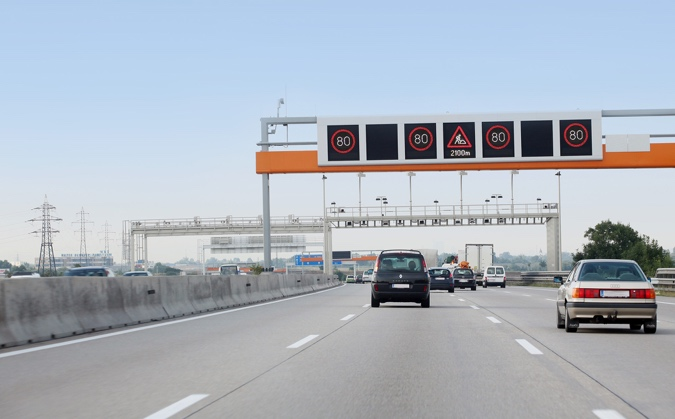
\includegraphics[width=2\linewidth]{image/dynamic_signage} \caption{Dynamic signage system in Austria (ASFiNAG, 2019b)}\label{fig:unnamed-chunk-4}
\end{figure}

With respect to the impact on the societal level, a Belgian study, by E. De Pauw et al.~showed a significant decrease (-18 \%) in the number of injury crashes after the introduction of a DSL system (De Pauw et al., 2018). F.G. Habtemichael and L. de Picado Santos (2013) found that a DSL system has the highest safety benefit during highly congested traffic conditions. The operational benefit in turn was the highest during lightly congested traffic conditions. However, the success of DSL is highly dependent on the level of driver compliance (Habtemichael \& de Picado Santos, 2013). Besides the safety aspects, the goal of DSL is to harmonize the traffic flow. Heavy traffic can cause shock waves, which result in longer travel times and large variations in the speeds of the vehicles. The latter again may lead to unsafe situations. By using DSL this phenomenon could be reduced (Hegyi et al., 2005). Traffic flow efficiency can be improved more, when DSL is combined with coordinated ramp metering (Carlson, 2010). Speed limits can also be temporary lowered, due to high emission values. If the emission values combined with the amount of traffic, reach a specific level, the DSL-System responds automatically and lowers the speed limit for a certain time. How high that level is, depends on the local policies (ASFiNAG, 2019c).

\hypertarget{key-stakeholders-2}{%
\subsection*{Key stakeholders}\label{key-stakeholders-2}}
\addcontentsline{toc}{subsection}{Key stakeholders}

\begin{itemize}
\tightlist
\item
  \textbf{Affected}: Motorways users
\item
  \textbf{Responsible}: Motorway Infrastructure Agencies, Technology Providers, Policymakers, State authorities
\end{itemize}

\hypertarget{current-state-of-art-in-research-2}{%
\subsection*{Current state of art in research}\label{current-state-of-art-in-research-2}}
\addcontentsline{toc}{subsection}{Current state of art in research}

Studies show, that in retrospect most DSL implementations in Europe were efficient traffic safety and flow improvement. In the United States the increase in safety was significant as well, but the flow improvement was controversial (Lu \& Shladover, 2014). Hassan et al.~(2012) discovered that during bad weather conditions the combination of Changeable Message Signs (CMS) and DSL was the best way to improve safety. Current research shows that the benefits of DSL systems could be improved by integrating it in a fully connected vehicles (CV) environment (Wu et al., 2020). Currently, research focuses on the integration of C-ITS, to connect the infrastructure to the vehicles. European standards should be developed during the next years (Erhart, 2019).

\hypertarget{current-state-of-art-in-practice-2}{%
\subsection*{Current state of art in practice}\label{current-state-of-art-in-practice-2}}
\addcontentsline{toc}{subsection}{Current state of art in practice}

DSL systems are implemented and used around the world. The used algorithms differ, however. DSL integrated with C-ITS has been implemented in a test environment (Erhart, 2019).
Austrian motorways are managed by the ASFiNAG - currently they have 17 DSL systems in use. That means that about 19 \% of the Austrian Motorway-System are currently equipped by an DSL system (ASFiNAG, 2019a). So, there is potential for expansion. One global player in traffic management is the Austrian company Kapsch TrafficCom. Worldwide they have implemented their systems on more than 3.500 km of motorway (Kapsch TrefficCom). Kapsch TrafficCom's approximately 5,000 employees generated revenues of EUR 738 million in the fiscal year 2018/19.

\hypertarget{relevant-initiatives-in-austria-2}{%
\subsection*{Relevant initiatives in Austria}\label{relevant-initiatives-in-austria-2}}
\addcontentsline{toc}{subsection}{Relevant initiatives in Austria}

\begin{itemize}
\tightlist
\item
  \href{https://www.asfinag.at/verkehrssicherheit/verkehrsmanagement/verkehrssteuerung/}{Asfinag}
\item
  \href{https://blog.asfinag.at/technik-innovation/c-its-vernetzte-autos-intelligenter-verkehr/}{Asifinag blog}
\item
  \href{https://www.kapsch.net/ktc/Portfolio/IMS/Congestion/Highway-Traffic-Management}{kapsch.net}
\item
  \href{https://www.strabag-iss.com/databases/internet/_public/content30.nsf/web30?Openagent\&id=DE-STRABAGISS-DE_verkehrstechnik.html\&men1=3\&men2=5\&sid=351}{strabag-iss.com}
\item
  \href{https://www.pke.at/index.php?id=17\#c117}{pke.at}
\item
  \href{http://www.aigner-stahlbau.at/leistungen/verkehrstechnik/}{aigner-stahlbau.at}
\end{itemize}

\hypertarget{impacts-with-respect-to-sustainable-development-goals-sdgs-2}{%
\subsection*{Impacts with respect to Sustainable Development Goals (SDGs)}\label{impacts-with-respect-to-sustainable-development-goals-sdgs-2}}
\addcontentsline{toc}{subsection}{Impacts with respect to Sustainable Development Goals (SDGs)}

\begin{longtable}[]{@{}ccccc@{}}
\toprule
\begin{minipage}[b]{0.17\columnwidth}\centering
Impact level\strut
\end{minipage} & \begin{minipage}[b]{0.16\columnwidth}\centering
Indicator\strut
\end{minipage} & \begin{minipage}[b]{0.17\columnwidth}\centering
Impact direction\strut
\end{minipage} & \begin{minipage}[b]{0.17\columnwidth}\centering
Goal description and number\strut
\end{minipage} & \begin{minipage}[b]{0.17\columnwidth}\centering
Source\strut
\end{minipage}\tabularnewline
\midrule
\endhead
\begin{minipage}[t]{0.17\columnwidth}\centering
Individual\strut
\end{minipage} & \begin{minipage}[t]{0.16\columnwidth}\centering
Fatal collisions reduced\strut
\end{minipage} & \begin{minipage}[t]{0.17\columnwidth}\centering
\textbf{+}\strut
\end{minipage} & \begin{minipage}[t]{0.17\columnwidth}\centering
Health \& Wellbeing (\emph{3})\strut
\end{minipage} & \begin{minipage}[t]{0.17\columnwidth}\centering
Hegyi et al., 2005\strut
\end{minipage}\tabularnewline
\begin{minipage}[t]{0.17\columnwidth}\centering
Individual\strut
\end{minipage} & \begin{minipage}[t]{0.16\columnwidth}\centering
Travel time reduced\strut
\end{minipage} & \begin{minipage}[t]{0.17\columnwidth}\centering
\textbf{+}\strut
\end{minipage} & \begin{minipage}[t]{0.17\columnwidth}\centering
Environmental sustainability (\emph{7,12-13,15})\strut
\end{minipage} & \begin{minipage}[t]{0.17\columnwidth}\centering
Habtemichael \& de Picado Santos, 2013\strut
\end{minipage}\tabularnewline
\begin{minipage}[t]{0.17\columnwidth}\centering
Systemic\strut
\end{minipage} & \begin{minipage}[t]{0.16\columnwidth}\centering
Fatal collisions reduced\strut
\end{minipage} & \begin{minipage}[t]{0.17\columnwidth}\centering
\textbf{+}\strut
\end{minipage} & \begin{minipage}[t]{0.17\columnwidth}\centering
Health \& Wellbeing (\emph{3})\strut
\end{minipage} & \begin{minipage}[t]{0.17\columnwidth}\centering
Hegyi et al., 2005\strut
\end{minipage}\tabularnewline
\begin{minipage}[t]{0.17\columnwidth}\centering
Systemic\strut
\end{minipage} & \begin{minipage}[t]{0.16\columnwidth}\centering
Annual greenhouse gas emissions decrease\strut
\end{minipage} & \begin{minipage}[t]{0.17\columnwidth}\centering
\textbf{+}\strut
\end{minipage} & \begin{minipage}[t]{0.17\columnwidth}\centering
Environmental sustainability (\emph{7,12-13,15})\strut
\end{minipage} & \begin{minipage}[t]{0.17\columnwidth}\centering
Schimany, 2011\strut
\end{minipage}\tabularnewline
\bottomrule
\end{longtable}

\hypertarget{technology-and-societal-readiness-level-2}{%
\subsection*{Technology and societal readiness level}\label{technology-and-societal-readiness-level-2}}
\addcontentsline{toc}{subsection}{Technology and societal readiness level}

\begin{longtable}[]{@{}cc@{}}
\toprule
TRL & SRL\tabularnewline
\midrule
\endhead
7-9 & 8-9\tabularnewline
\bottomrule
\end{longtable}

\hypertarget{open-questions-2}{%
\subsection*{Open questions}\label{open-questions-2}}
\addcontentsline{toc}{subsection}{Open questions}

\begin{enumerate}
\def\labelenumi{\arabic{enumi}.}
\tightlist
\item
  Which algorithms for DSL are the most efficient ones?
\item
  How can DSL be further developed?
\item
  How can fail-safe operation be improved?
\item
  How can DSL be combined with C-ITS?
\end{enumerate}

\hypertarget{references-2}{%
\subsection*{References}\label{references-2}}
\addcontentsline{toc}{subsection}{References}

\begin{itemize}
\tightlist
\item
  ASFiNAG. (2019a). Handlungsfelder. Retrieved 17th December 2020, from \url{http://verkehrssicherheit.asfinag.at/aktionsprogramme/handlungsfelder/}
\item
  ASFiNAG. (2019b). Verkehrsbeeinflussungsanlagen -- Für mehr Sicherheit: Arten von Verkehrsbeeinflussungsanlagen. Retrieved 11th December 2020, from \url{https://asfinag.azureedge.net/media/1607/vba-fotomontage.jpg}
\item
  ASFiNAG. (2019c). Verkehrsbeeinflussungsanlagen -- Für mehr Sicherheit: Die VBA und der ``Lufthunderter''. Retrieved 3rd December 2020, from \url{https://www.asfinag.at/verkehrssicherheit/verkehrsmanagement/verkehrssteuerung/}
\item
  Carlson, R. C., Papamichail, I., Papageorgiou, M., \& Messmer, A. (2010). Optimal motorway traffic flow control involving variable speed limits and ramp metering. Transportation Science, 44(2), 238-253.
\item
  De Pauw, E., Daniels, S., Franckx, L., \& Mayeres, I. (2018). Safety effects of dynamic speed limits on motorways. Accident Analysis \& Prevention, 114, 83-89.
\item
  Erhart, Jaqueline. (2019). Vernetzte Autos, intelligenter Verkehr: Was C-ITS ist, was es kann und wem es nutzt. Retrieved 17th December 2020, from \url{https://blog.asfinag.at/technik-innovation/c-its-vernetzte-autos-intelligenter-verkehr/}\\
\item
  Habtemichael, F. G., \& de Picado Santos, L. (2013). Safety and Operational Benefits of Variable Speed Limits under Different Traffic Conditions and Driver Compliance Levels. Transportation Research Record, 2386(1), 7--15. \url{https://doi.org/10.3141/2386-02}
\item
  Hassan, H. M., Abdel-Aty, M. A., Choi, K., \& Algadhi, S. A. (2012). Driver behavior and preferences for changeable message signs and variable speed limits in reduced visibility conditions. Journal of Intelligent Transportation Systems, 16(3), 132-146.
\item
  Hegyi, A., De Schutter, B., \& Hellendoorn, J. (2005). Optimal coordination of variable speed limits to suppress shock waves. IEEE Transactions on intelligent transportation systems, 6(1), 102-112.
\item
  Kapsch TrefficCom. Verkehrsmanagement auf Autobahnen. Retrieved 8th January 2021, \url{https://www.kapsch.net/ktc/Portfolio/IMS/Congestion/Highway-Traffic-Management}
\item
  Lu, X.-Y., \& Shladover, S. E. (2014). Review of Variable Speed Limits and Advisories: Theory, Algorithms, and Practice. Transportation Research Record, 2423(1), 15--23. \url{https://doi.org/10.3141/2423-03}
\item
  Mobility and Transport \textbar{} European Commission. (2020). Dynamic speed limits. Retrieved 2nd December 2020, from \url{https://ec.europa.eu/transport/road_safety/specialist/knowledge/speed/new_technologies_new_opportunities/dynamic_speed_limits_en}
\item
  Schimany, H. K. (2011). Blue Globe Foresight.
\item
  Wu, Y., Abdel-Aty, M., Wang, L., \& Rahman, M. S. (2020). Combined connected vehicles and variable speed limit strategies to reduce rear-end crash risk under fog conditions. Journal of Intelligent Transportation Systems, 24(5), 494-513.
\end{itemize}

\hypertarget{passengers-and-goods-fleet-management}{%
\section{Passengers and goods fleet management}\label{passengers-and-goods-fleet-management}}

\hypertarget{urban-access-management}{%
\section{Urban access management}\label{urban-access-management}}

\hypertarget{pricing}{%
\chapter{Road pricing}\label{pricing}}

\hypertarget{congestion-charging}{%
\section{Congestion charging}\label{congestion-charging}}

\hypertarget{digital}{%
\chapter{Digital road infrastructure and connectivity}\label{digital}}

\hypertarget{vehicle-to-infrastructure-communication}{%
\section{Vehicle to infrastructure communication}\label{vehicle-to-infrastructure-communication}}

\hypertarget{infrastructure-support-levels-for-automated-driving}{%
\section{Infrastructure support levels for automated driving}\label{infrastructure-support-levels-for-automated-driving}}

\hypertarget{vehicle-to-vehicle-communication}{%
\section{Vehicle to vehicle communication}\label{vehicle-to-vehicle-communication}}

\hypertarget{wireless-communication}{%
\section{Wireless communication}\label{wireless-communication}}

\hypertarget{passenger}{%
\chapter{Passenger information system}\label{passenger}}

\hypertarget{digital-journey-planner}{%
\section{Digital journey planner}\label{digital-journey-planner}}

\hypertarget{rail-telematics-for-passenger-services}{%
\section{Rail telematics for passenger services}\label{rail-telematics-for-passenger-services}}

\hypertarget{multimodal-information-and-route-planning}{%
\section{Multimodal information and route planning}\label{multimodal-information-and-route-planning}}

\hypertarget{real-time-location-based-information}{%
\section{Real-time, location-based information}\label{real-time-location-based-information}}

\hypertarget{multimodal}{%
\chapter{Multimodal integrated system}\label{multimodal}}

\hypertarget{first-last-mile-solutions}{%
\section{First-last mile solutions}\label{first-last-mile-solutions}}

\hypertarget{distance-or-time-based-fares}{%
\section{Distance or time-based fares}\label{distance-or-time-based-fares}}

\hypertarget{mobility-as-a-service}{%
\section{Mobility as a service}\label{mobility-as-a-service}}

\hypertarget{park-and-ride}{%
\section{Park and ride}\label{park-and-ride}}

\hypertarget{contantless-public-transport-cards}{%
\section{Contantless public transport cards}\label{contantless-public-transport-cards}}

\hypertarget{information-and-assistance-for-people-with-special-needs}{%
\section{Information and assistance for people with special needs}\label{information-and-assistance-for-people-with-special-needs}}

\hypertarget{mobilityfreight-hubs}{%
\section{Mobility/Freight hubs}\label{mobilityfreight-hubs}}

\hypertarget{connected}{%
\chapter{Connected and autonomous driving}\label{connected}}

\hypertarget{parking-infrastructure-for-autonomous-vehicles}{%
\section{Parking infrastructure for autonomous vehicles}\label{parking-infrastructure-for-autonomous-vehicles}}

\hypertarget{connected-vehicles}{%
\section{Connected vehicles}\label{connected-vehicles}}

\hypertarget{automated-vehicles}{%
\section{Automated vehicles}\label{automated-vehicles}}

\hypertarget{onboard}{%
\chapter{On-board technology for connected and automated vehicles}\label{onboard}}

\hypertarget{advanced-driver-assistance-system}{%
\section{Advanced driver assistance system}\label{advanced-driver-assistance-system}}

\hypertarget{parking-assistance-system}{%
\section{Parking assistance system}\label{parking-assistance-system}}

\hypertarget{lane-keeping}{%
\section{Lane keeping}\label{lane-keeping}}

\hypertarget{distane-keeping}{%
\section{Distane keeping}\label{distane-keeping}}

\hypertarget{crash-avoidance}{%
\section{Crash avoidance}\label{crash-avoidance}}

\hypertarget{mainteinance-assistance}{%
\section{Mainteinance assistance}\label{mainteinance-assistance}}

\hypertarget{digital-maps}{%
\section{Digital maps}\label{digital-maps}}

\hypertarget{e-horizon}{%
\section{E-Horizon}\label{e-horizon}}

\hypertarget{emergency-call}{%
\section{Emergency call}\label{emergency-call}}

\hypertarget{freight}{%
\chapter{Freight and commercial transport}\label{freight}}

\hypertarget{automated-road-freight}{%
\section{Automated road freight}\label{automated-road-freight}}

\hypertarget{freight-dreyage-optimisation}{%
\section{Freight dreyage optimisation}\label{freight-dreyage-optimisation}}

\hypertarget{tracking-and-tracing-of-dangerous-goods}{%
\section{Tracking and tracing of dangerous goods}\label{tracking-and-tracing-of-dangerous-goods}}

\hypertarget{intermodal-freight}{%
\section{Intermodal Freight}\label{intermodal-freight}}

\hypertarget{real-time-disruption-management-and-route-planning}{%
\section{Real-time disruption management and route planning}\label{real-time-disruption-management-and-route-planning}}

\hypertarget{traffic-signal-control}{%
\section{Traffic signal control}\label{traffic-signal-control}}

\hypertarget{urban-deliveries}{%
\section{Urban Deliveries}\label{urban-deliveries}}

\hypertarget{parcel-load-pooling}{%
\section{Parcel load pooling}\label{parcel-load-pooling}}

\hypertarget{intelligent-truck-parking-and-delivery-space-booking}{%
\section{Intelligent truck parking and delivery space booking}\label{intelligent-truck-parking-and-delivery-space-booking}}

\hypertarget{freight-drones}{%
\section{Freight drones}\label{freight-drones}}

\hypertarget{commercial-vehicle-on-board-safety-systems}{%
\section{Commercial vehicle on-board safety systems}\label{commercial-vehicle-on-board-safety-systems}}

\hypertarget{truck-platooning}{%
\section{Truck Platooning}\label{truck-platooning}}

\hypertarget{rail-telematics-for-freight-services}{%
\section{Rail telematics for freight services}\label{rail-telematics-for-freight-services}}

\hypertarget{electric-vehicle-delivery-fleets}{%
\section{Electric vehicle delivery fleets}\label{electric-vehicle-delivery-fleets}}

\hypertarget{multimodal-transport-management-systems}{%
\section{Multimodal transport management systems}\label{multimodal-transport-management-systems}}

\hypertarget{cooperative-adaptive-cruise-control-in-trucks}{%
\section{Cooperative adaptive cruise control in trucks}\label{cooperative-adaptive-cruise-control-in-trucks}}

\hypertarget{collective}{%
\chapter{Collective mobility vehicles}\label{collective}}

\hypertarget{demand-responsive-transit}{%
\section{Demand responsive transit}\label{demand-responsive-transit}}

\hypertarget{personal-rapid-transit}{%
\section{Personal rapid transit}\label{personal-rapid-transit}}

\hypertarget{bus-rapid-transit}{%
\section{Bus rapid transit}\label{bus-rapid-transit}}

\hypertarget{light-rail-transit}{%
\section{Light rail transit}\label{light-rail-transit}}

\hypertarget{passenger-drones}{%
\section{Passenger drones}\label{passenger-drones}}

\hypertarget{automatic-train-operations}{%
\section{Automatic train operations}\label{automatic-train-operations}}

\hypertarget{big}{%
\chapter{Big data}\label{big}}

\hypertarget{automatic-identification-system-fir-maritime-transport}{%
\section{Automatic identification system fir maritime transport}\label{automatic-identification-system-fir-maritime-transport}}

\hypertarget{big-data-lifecycle}{%
\section{Big data lifecycle}\label{big-data-lifecycle}}

\hypertarget{location-based-data}{%
\section{Location-based data}\label{location-based-data}}

\hypertarget{aircraft-tracking-system}{%
\section{Aircraft tracking system}\label{aircraft-tracking-system}}

\hypertarget{big-data-tools-for-maping-and-forecasting-travel-behaviour}{%
\section{Big data tools for maping and forecasting travel behaviour}\label{big-data-tools-for-maping-and-forecasting-travel-behaviour}}

\hypertarget{shared}{%
\chapter{Shared mobility}\label{shared}}

\hypertarget{car-sharing}{%
\section{Car sharing}\label{car-sharing}}

\hypertarget{synonyms-3}{%
\subsection*{Synonyms}\label{synonyms-3}}
\addcontentsline{toc}{subsection}{Synonyms}

\emph{Car-Sharing scheme, CSS}

\hypertarget{definition-3}{%
\subsection*{Definition}\label{definition-3}}
\addcontentsline{toc}{subsection}{Definition}

In recent years, the growth of car sharing services as a new and more sustainable way of travelling has led to a shift in private mobility from ownership to use of services. The basic idea of car sharing is quite simple: the sharing of a fleet of vehicles by members to make trips on a per-trip basis. Although, the first car sharing scheme for economic reasons dates back to 1948 in the city of Zurich, Switzerland, other attempts at public car sharing schemes in the following years were not successful. Several successful car sharing schemes were launched in the 1980s, with a consolidation in the early 1990s, thanks to an increasing awareness of citizens and a real boom due to a greater diffusion of ICT and mobile services in the 2000s. Car sharing increases the mobility of community members to reach destinations otherwise inaccessible by public transport, walking or cycling, while raising citizens' awareness of the social and environmental impacts of using private cars. It encourages and supports multimodal communities by providing an additional transport option. From the point of view of building a sustainable city, the vehicles used in car sharing are usually fuel efficient and lead to positive effects in reducing urban emissions and urban congestion (Martin and Shaheen, 2011).

Nowadays, there are different variants of car sharing available on the market. These include:

\begin{itemize}
\tightlist
\item
  Station based
\end{itemize}

In station-based CarSharing, the cars are parked in fixed parking spaces as close to home as possible. Customers pick up the car there and return it after the journey. Only with this variant, the reservations are possible several days or weeks in advance, but the end time of the booking must also usually be planned in advance. This ensures a high degree of predictability in vehicle availability. Station-based CarSharing is also the cheapest CarSharing variant. The largest providers in Germany (by fleet size) are stadtmobil, cambio, teilAuto and book-n-drive.

\begin{itemize}
\tightlist
\item
  Free-floating
\end{itemize}

With free-floating CarSharing, the cars are randomly distributed within a defined business area. Users locate and book them via smartphone. The booking is only possible shortly before the start of the journey and until booking, availability and exact location of the vehicle are uncertain. After the journey, the cars can be parked within the business area. All bookings are open-ended. With this variant, reservations in advance are not possible. Both the availability and the location of the vehicle are therefore difficult to predict. Free-floating, however, allows one-way journeys within the business area. Prices are higher than those of station-based CarSharing. The largest providers in Germany are ShareNow, Sixt share and We share.

\begin{itemize}
\tightlist
\item
  Combined sharing
\end{itemize}

Since 2011, combined CarSharing offers were established that offer station-based and free-floating vehicles from a single source. Combined offers in Germany are available, for example, from stadtmobil, book-n-drive, teilAuto and cambio. The prices are usually based on the lower prices of station-based CarSharing.
Free-floating users, on the other hand, largely keep their car. Their motorisation at the time of the study was 485 private cars per 1,000 inhabitants (Bundesverband CarSharing e.V., 2020).

\hypertarget{key-stakeholders-3}{%
\subsection*{Key stakeholders}\label{key-stakeholders-3}}
\addcontentsline{toc}{subsection}{Key stakeholders}

\begin{itemize}
\tightlist
\item
  \textbf{Affected}: Citizens
\item
  \textbf{Responsible}: Authorities, Municipalities, International lobbyists, Private Companies
\end{itemize}

\hypertarget{current-state-of-art-in-research-3}{%
\subsection*{Current state of art in research}\label{current-state-of-art-in-research-3}}
\addcontentsline{toc}{subsection}{Current state of art in research}

The CarSharing variants have different traffic-reducing effects. The EU research project STARS investigated the traffic-relieving effect of different CarSharing variants under uniform framework conditions. The study shows that many users of station-based and combined CarSharing get rid of private cars shortly before or during CarSharing participation. At the time of the study, the households, therefore, only had a motorisation rate of 108 and 104 cars per 1,000 people in the surveyed households. These values are already below the target of 150 cars per 1,000 people recommended by the Federal Environment Agency Germany for climate and environmentally friendly urban transport in the future.

The replacement rates in different CarSharing studies from Germany vary. On the one hand, this is due to different survey methods. Only in the studies since 2018 have used a largely uniform survey method in Germany. On the other hand, the latest research has shown that the replacement rate depends strongly on the CarSharing variant studied. For station-based CarSharing and combined CarSharing, there are exclusively positive replacement rates. For pure free-floating CarSharing, both positive and negative replacement rates can be observed. In some cases, fewer private cars were removed by free-floating CarSharing than were put on the road by the CarSharing service.

According to calculations made by Finanztip together with the ADAC, car sharing is already profitable if the number of kilometres driven per year is less than 10,000, or less than 800 kilometres per month. The costs for a private vehicle with 10,000 annual kilometres driven are identical to the costs that would be incurred for car sharing. Other studies see the limit only at 11,250 kilometres (Hoyer, 2013) or 15,600 kilometres (Seipp, 2014). At 5,000 kilometres per year with one's own medium-sized vehicle, one would save on average between 900 and 1,500 euros per year with a car-sharing provider.
In summary, accrding to Evers (2018) car sharing is profitable, if one:

\begin{itemize}
\tightlist
\item
  does not depend on a car every day
\item
  does not regularly drive longer distances over 100 kilometres
\item
  drives a total of less than 10,000 kilometres a year
\end{itemize}

\hypertarget{current-state-of-art-in-practice-3}{%
\subsection*{Current state of art in practice}\label{current-state-of-art-in-practice-3}}
\addcontentsline{toc}{subsection}{Current state of art in practice}

Europe is currently the most important market for car sharing providers. In 2016, 5.8 million people used the 68,000 carsharing vehicles here. Recently, car manufacturers also started to enter the market directly, such as Daimler, BMW and the FCA Group, which are directly involved in car sharing activities, in order to find new channels to market the cars they produce. The market is growing fast and with this increasing demand comes the need for better understanding and control of the system. In fact, car sharing is not just a matter of business or fleet optimisation, but forms a complex system consisting of different actors, including citizens, authorities and municipalities, businesses. The system becomes complex because of the strong links between the actors as well as the impact on the governance of a city when a large car sharing service is introduced, such as the integration with the existing public transport network and the policies that allow different companies to compete in the same urban area (Ferrero et al., 2018).

\hypertarget{relevant-initiatives-in-austria-3}{%
\subsection*{Relevant initiatives in Austria}\label{relevant-initiatives-in-austria-3}}
\addcontentsline{toc}{subsection}{Relevant initiatives in Austria}

\begin{itemize}
\tightlist
\item
  \href{https://www.vcoe.at/presse/presseaussendungen/detail/carsharing-haushalte-potential-2018}{VCÖ}
\item
  \href{https://www.carsharing-wien.com/anbieter/oebb-rail-and-drive}{ÖBB}
\end{itemize}

\hypertarget{impacts-with-respect-to-sustainable-development-goals-sdgs-3}{%
\subsection*{Impacts with respect to Sustainable Development Goals (SDGs)}\label{impacts-with-respect-to-sustainable-development-goals-sdgs-3}}
\addcontentsline{toc}{subsection}{Impacts with respect to Sustainable Development Goals (SDGs)}

\begin{longtable}[]{@{}ccccc@{}}
\toprule
\begin{minipage}[b]{0.17\columnwidth}\centering
Impact level\strut
\end{minipage} & \begin{minipage}[b]{0.16\columnwidth}\centering
Indicator\strut
\end{minipage} & \begin{minipage}[b]{0.17\columnwidth}\centering
Impact direction\strut
\end{minipage} & \begin{minipage}[b]{0.17\columnwidth}\centering
Goal description and number\strut
\end{minipage} & \begin{minipage}[b]{0.17\columnwidth}\centering
Source\strut
\end{minipage}\tabularnewline
\midrule
\endhead
\begin{minipage}[t]{0.17\columnwidth}\centering
Individual\strut
\end{minipage} & \begin{minipage}[t]{0.16\columnwidth}\centering
Uniform access to car in the population\strut
\end{minipage} & \begin{minipage}[t]{0.17\columnwidth}\centering
\textbf{+}\strut
\end{minipage} & \begin{minipage}[t]{0.17\columnwidth}\centering
Equality (\emph{5,10})\strut
\end{minipage} & \begin{minipage}[t]{0.17\columnwidth}\centering
VCOE - Mobilitaet mit Zukunft, 2018\strut
\end{minipage}\tabularnewline
\begin{minipage}[t]{0.17\columnwidth}\centering
Individual\strut
\end{minipage} & \begin{minipage}[t]{0.16\columnwidth}\centering
Cost reduced\strut
\end{minipage} & \begin{minipage}[t]{0.17\columnwidth}\centering
\textbf{+}\strut
\end{minipage} & \begin{minipage}[t]{0.17\columnwidth}\centering
Sustainable economic development (\emph{8,11})\strut
\end{minipage} & \begin{minipage}[t]{0.17\columnwidth}\centering
Evers, 2018\strut
\end{minipage}\tabularnewline
\begin{minipage}[t]{0.17\columnwidth}\centering
Systemic\strut
\end{minipage} & \begin{minipage}[t]{0.16\columnwidth}\centering
Reduced traffic and improved air quality\strut
\end{minipage} & \begin{minipage}[t]{0.17\columnwidth}\centering
\textbf{+}\strut
\end{minipage} & \begin{minipage}[t]{0.17\columnwidth}\centering
Health \& Wellbeing (\emph{3})\strut
\end{minipage} & \begin{minipage}[t]{0.17\columnwidth}\centering
Martin and Shaheen, 2011\strut
\end{minipage}\tabularnewline
\begin{minipage}[t]{0.17\columnwidth}\centering
Systemic\strut
\end{minipage} & \begin{minipage}[t]{0.16\columnwidth}\centering
Car-free households are no longer disadvantaged\strut
\end{minipage} & \begin{minipage}[t]{0.17\columnwidth}\centering
\textbf{+}\strut
\end{minipage} & \begin{minipage}[t]{0.17\columnwidth}\centering
Equality (\emph{5,10})\strut
\end{minipage} & \begin{minipage}[t]{0.17\columnwidth}\centering
VCOE - Mobiliteat mit Zukunft, 2018\strut
\end{minipage}\tabularnewline
\begin{minipage}[t]{0.17\columnwidth}\centering
Systemic\strut
\end{minipage} & \begin{minipage}[t]{0.16\columnwidth}\centering
Reduced emissions\strut
\end{minipage} & \begin{minipage}[t]{0.17\columnwidth}\centering
\textbf{+}\strut
\end{minipage} & \begin{minipage}[t]{0.17\columnwidth}\centering
Environmental sustainability (\emph{7,12-13,15})\strut
\end{minipage} & \begin{minipage}[t]{0.17\columnwidth}\centering
Martin and Shaheen, 2011\strut
\end{minipage}\tabularnewline
\begin{minipage}[t]{0.17\columnwidth}\centering
Systemic\strut
\end{minipage} & \begin{minipage}[t]{0.16\columnwidth}\centering
Car sharing fleet grows steadily\strut
\end{minipage} & \begin{minipage}[t]{0.17\columnwidth}\centering
\textbf{+}\strut
\end{minipage} & \begin{minipage}[t]{0.17\columnwidth}\centering
Innovation \& Infrastructure (\emph{9})\strut
\end{minipage} & \begin{minipage}[t]{0.17\columnwidth}\centering
Stadt Wien, Strassenverwaltung und Strassenbau, no date\strut
\end{minipage}\tabularnewline
\bottomrule
\end{longtable}

\hypertarget{technology-and-societal-readiness-level-3}{%
\subsection*{Technology and societal readiness level}\label{technology-and-societal-readiness-level-3}}
\addcontentsline{toc}{subsection}{Technology and societal readiness level}

\begin{longtable}[]{@{}cc@{}}
\toprule
TRL & SRL\tabularnewline
\midrule
\endhead
7-9 & 5-7\tabularnewline
\bottomrule
\end{longtable}

\hypertarget{open-questions-3}{%
\subsection*{Open questions}\label{open-questions-3}}
\addcontentsline{toc}{subsection}{Open questions}

\begin{enumerate}
\def\labelenumi{\arabic{enumi}.}
\tightlist
\item
  What is the role of policymakers and minicipalities in supporting car sharing in addressing challenges associated with long-term strategic decisions such as operation area, parking locations or size and type of the fleet, considering specific characteristics of a given city?
\end{enumerate}

\hypertarget{further-links-2}{%
\subsection*{Further links}\label{further-links-2}}
\addcontentsline{toc}{subsection}{Further links}

\begin{itemize}
\tightlist
\item
  \href{https://www.share-now.com/at/en/faq/}{share\_now}
\end{itemize}

\hypertarget{references-3}{%
\subsection*{References}\label{references-3}}
\addcontentsline{toc}{subsection}{References}

\begin{itemize}
\tightlist
\item
  Bundesverband CarSharing (2020) CarSharing in Deutschland 2020.
\item
  Bundesverband CarSharing e.V. (2020) Verkehrsentlastung durch CarSharing - Factsheet.
\item
  Evers, H. (2018) Carsharing günstiger als eigenes Auto? Available at: \url{https://www.computerbild.de/artikel/cb-Tipps-Connected-Car-Kostenvergleich-Ab-wann-lohnt-sich-Carsharing-20041131.html} (Accessed: 14 January 2021).
\item
  Ferrero, F. et al.~(2018) `Car-sharing services: An annotated review', Sustainable Cities and Society, 37, pp.~501--518. doi: \url{https://doi.org/10.1016/j.scs.2017.09.020}.
\item
  Hoyer, N. (2013) Mobilität: Lohnt sich Ihr Auto? Available at: \url{https://www.wiwo.de/technologie/mobilitaet/mobilitaet-lohnt-sich-ihr-auto/8681062-all.html} (Accessed: 14 January 2021).
\item
  Martin, E. W. and Shaheen, S. A. (2011) `Greenhouse Gas Emission Impacts of Carsharing in North America', IEEE Transactions on Intelligent Transportation Systems, 12(4), pp.~1074--1086. doi: 10.1109/TITS.2011.2158539.
\item
  Seipp, B. (2014) Carsharing: Für wen sich das geteilte Auto wirklich lohnt - WELT. Available at: \url{https://www.welt.de/motor/article128304929/Fuer-wen-sich-das-geteilte-Auto-wirklich-lohnt.html} (Accessed: 14 January 2021).
\item
  Stadt Wien \textbar{} Straßenverwaltung und Straßenbau (no date) Carsharing in Wien: Nutzung nimmt zu. Available at: \url{https://www.wien.gv.at/verkehr/kfz/carsharing/evaluierung.html} (Accessed: 17 January 2021).
\item
  VCÖ - Mobilität mit Zukunft (2018) Mehr als 100.000 Carsharing-Haushalte in Österreich -- Potenzial um ein Vielfaches höher - Mobilität mit Zukunft. Available at: \url{https://www.vcoe.at/presse/presseaussendungen/detail/carsharing-haushalte-potential-2018} (Accessed: 18 January 2021).
\end{itemize}

\hypertarget{bicycle-and-e-bicycle-hire}{%
\section{Bicycle and e-bicycle hire}\label{bicycle-and-e-bicycle-hire}}

\hypertarget{e-scooter-hire}{%
\section{E-scooter hire}\label{e-scooter-hire}}

\hypertarget{ride-hailing}{%
\section{Ride-hailing}\label{ride-hailing}}

\hypertarget{alternative}{%
\chapter{Alternative power sources}\label{alternative}}

\hypertarget{hydrogen-fuel-cell}{%
\section{Hydrogen fuel cell}\label{hydrogen-fuel-cell}}

\hypertarget{definition-4}{%
\subsection*{Definition}\label{definition-4}}
\addcontentsline{toc}{subsection}{Definition}

Hydrogen Fuel Cells are systems that use hydrogen as fuel to generate electrical energy in a Fuel Cell and drive the vehicle with electrical structure. In a technical manner, they show similarities with electric vehicles. The advantages of Fuel Cell Electrical Vehicles (FCEV) are emission-free (water only), fast refuelling, noiseless driving, more economical fuel consumption and efficiency, easy maintenance. Regardless of these benefits, FCEV has some disadvantages, such as limited range, lack of hydrogen refuelling stations, safety problems, low profitability for car manufacturers, high prices and lower awareness and acceptance (Tanç et al., 2019; Borgstedt et al., 2017; Iribarren et al., 2016). Moreover, FCEVs have higher energy density than electric batteries which enables them to drive further with heavier loads. At the same time, it raises constraints on weight and size of the energy storage in the vehicles. Consequently, FCEVs are more suitable for freight transport, commercial vehicles, buses, trains, ships and aircrafts, where the performance requirements are higher. Prototypes of all the examples mentioned already exist (Eichlseder et al, 2018). In terms of private cars, the FCEVs are likely to provide advantage for long-distance travelling (Roadmap Europe, 2019).

\hypertarget{key-stakeholders-4}{%
\subsection*{Key stakeholders}\label{key-stakeholders-4}}
\addcontentsline{toc}{subsection}{Key stakeholders}

\begin{itemize}
\tightlist
\item
  \textbf{Affected}: Conventional Cars' Drivers, Citizen
\item
  \textbf{Responsible}: National Governments, Car Manufacturers, International lobbyists, Private Companies
\end{itemize}

\hypertarget{current-state-of-art-in-research-4}{%
\subsection*{Current state of art in research}\label{current-state-of-art-in-research-4}}
\addcontentsline{toc}{subsection}{Current state of art in research}

The goal of alternative propulsion systems is to minimize or eliminate completely the climate-damaging CO\textsubscript{2} emissions, consequently the European Community Research Program proposes electromobility as a priority research area. In particular, the most substantial research is carried out on methods of hydrogen production using biological and photochemical processes because 95\% of hydrogen currently produced on an industrial scale comes from fossil hydrocarbons and only 5\% from water by electrolysis. Where the only emission-free production process of hydrogen is the electrochemical water splitting in electrolysis, when the required electricity is generated from wind-, water or solar energy. This process results in high degrees of purity and usually achieves efficiencies of up to 85\% (Eichlseder et al., 2018). Moreover, the electric vehicle policy aims at technology optimization, market development, durability and capacity of the batteries and charging stations (Alvarez-Meaza et al., 2020).

\hypertarget{current-state-of-art-in-practice-4}{%
\subsection*{Current state of art in practice}\label{current-state-of-art-in-practice-4}}
\addcontentsline{toc}{subsection}{Current state of art in practice}

Hydrogen in transport is only at the beginning of its development (in 2013 the first light FCEVs were introduced for leasing only). Compared to other alternative propulsion systems such as battery electric vehicles (BEVs), which were introduced to the vehicle market earlier, FCEVs show a similar upward trend. At the end of 2017, the total number of FCEVs in Europe reached 799 vehicles, of which 602 were passenger cars and 197 light commercial vehicles, while the total number of BEVs reached 447,150 vehicles. At the end of 2018, the number of FCEVs in Europe rose to about 1,110 (Apostolou and Xydis, 2019).
At the end of October 2019, 41 fuel cell passenger cars were registered in Austria. Worldwide, about 12,900 fuel cell vehicles were in operation at the end of 2018, 11,200 of them passenger cars. 46 percent of the vehicles are on the road in the USA, 43 percent in Asia and 11 percent in the EU (1,110 cars). In terms of commercial vehicles, China dominates with over 400 buses, followed by the USA with 55 and the EU with around 80 (Eichlseder et al., 2018).
In terms of the number of hydrogen refuelling stations (HRS) worldwide, just about 375 stations are in operation today, compared to 320 in 2017. Most of these are publicly available, the rest are demonstration/research projects and are used to supply hydrogen to private fleets. At the end of 2018, Europe was the region with the most HRS in operation with more than 170 HRS, while Asia (mainly Japan) was second with about 130 HRS and America (mainly the US) third with more than 70 stations installed. Figure below shows the number of HRS by country at the end of 2018 (Apostolou and Xydis, 2019):

\begin{figure}
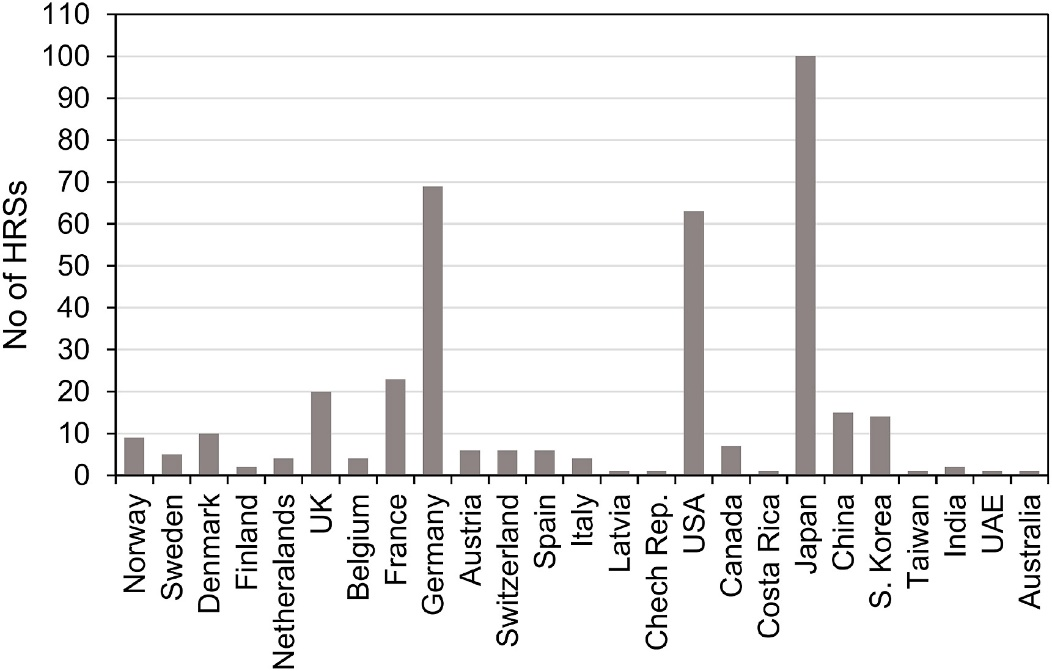
\includegraphics[width=2\linewidth]{image/hydrogen_refuel} \caption{Number of hydrogen refuelling stations worldwide (Apostolou and Xydis, 2019)}\label{fig:unnamed-chunk-5}
\end{figure}

The European Strategic Energy Technology Plan proposes hydrogen and fuel-cell technologies as crucial for obtaining green-house gases reduction goals by 2050 (Roadmap Europe H. 2019, Alvarez-Meaza et al., 2020).

\hypertarget{relevant-initiatives-in-austria-4}{%
\subsection*{Relevant initiatives in Austria}\label{relevant-initiatives-in-austria-4}}
\addcontentsline{toc}{subsection}{Relevant initiatives in Austria}

\begin{itemize}
\tightlist
\item
  \href{https://fuelcellsworks.com/news/alstoms-hydrogen-train-successfully-completes-three-months-of-testing-in-austria/\#:~:text=Alstom's\%20Hydrogen\%20Train\%20Successfully\%20Completes\%20Three\%20Months\%20of\%20Testing\%20in\%20Austria,-By\%20FuelCellsWorksDecember\&text=Alstom's\%20Coradia\%20iLint\%2C\%20the\%20world's,Austrian\%20Federal\%20Railways}{hydrogen train}
\end{itemize}

\hypertarget{impacts-with-respect-to-sustainable-development-goals-sdgs-4}{%
\subsection*{Impacts with respect to Sustainable Development Goals (SDGs)}\label{impacts-with-respect-to-sustainable-development-goals-sdgs-4}}
\addcontentsline{toc}{subsection}{Impacts with respect to Sustainable Development Goals (SDGs)}

\begin{longtable}[]{@{}ccccc@{}}
\toprule
\begin{minipage}[b]{0.17\columnwidth}\centering
Impact level\strut
\end{minipage} & \begin{minipage}[b]{0.16\columnwidth}\centering
Indicator\strut
\end{minipage} & \begin{minipage}[b]{0.17\columnwidth}\centering
Impact direction\strut
\end{minipage} & \begin{minipage}[b]{0.17\columnwidth}\centering
Goal description and number\strut
\end{minipage} & \begin{minipage}[b]{0.17\columnwidth}\centering
Source\strut
\end{minipage}\tabularnewline
\midrule
\endhead
\begin{minipage}[t]{0.17\columnwidth}\centering
Individual\strut
\end{minipage} & \begin{minipage}[t]{0.16\columnwidth}\centering
Improved air quality\strut
\end{minipage} & \begin{minipage}[t]{0.17\columnwidth}\centering
\textbf{+}\strut
\end{minipage} & \begin{minipage}[t]{0.17\columnwidth}\centering
Health \& Wellbeing (\emph{3})\strut
\end{minipage} & \begin{minipage}[t]{0.17\columnwidth}\centering
Colella, Jacobson and Golden, 2005\strut
\end{minipage}\tabularnewline
\begin{minipage}[t]{0.17\columnwidth}\centering
Individual\strut
\end{minipage} & \begin{minipage}[t]{0.16\columnwidth}\centering
High prices of hydrogen cars and hydrogen fuel\strut
\end{minipage} & \begin{minipage}[t]{0.17\columnwidth}\centering
\textbf{-}\strut
\end{minipage} & \begin{minipage}[t]{0.17\columnwidth}\centering
Equality (\emph{5,10})\strut
\end{minipage} & \begin{minipage}[t]{0.17\columnwidth}\centering
Kanna and Paturu, 2020\strut
\end{minipage}\tabularnewline
\begin{minipage}[t]{0.17\columnwidth}\centering
Individual\strut
\end{minipage} & \begin{minipage}[t]{0.16\columnwidth}\centering
Cost for individuals\strut
\end{minipage} & \begin{minipage}[t]{0.17\columnwidth}\centering
\textbf{\textasciitilde{}}\strut
\end{minipage} & \begin{minipage}[t]{0.17\columnwidth}\centering
Sustainable economic development (\emph{8,11})\strut
\end{minipage} & \begin{minipage}[t]{0.17\columnwidth}\centering
Apostolou and Xydis, 2019\strut
\end{minipage}\tabularnewline
\begin{minipage}[t]{0.17\columnwidth}\centering
Systemic\strut
\end{minipage} & \begin{minipage}[t]{0.16\columnwidth}\centering
Emissions reduced, improved air quality\strut
\end{minipage} & \begin{minipage}[t]{0.17\columnwidth}\centering
\textbf{+}\strut
\end{minipage} & \begin{minipage}[t]{0.17\columnwidth}\centering
Health \& Wellbeing (\emph{3})\strut
\end{minipage} & \begin{minipage}[t]{0.17\columnwidth}\centering
Colella, Jacobson and Golden, 2005\strut
\end{minipage}\tabularnewline
\begin{minipage}[t]{0.17\columnwidth}\centering
Systemic\strut
\end{minipage} & \begin{minipage}[t]{0.16\columnwidth}\centering
Distribution and allocation of goods worsens\strut
\end{minipage} & \begin{minipage}[t]{0.17\columnwidth}\centering
\textbf{-}\strut
\end{minipage} & \begin{minipage}[t]{0.17\columnwidth}\centering
Equality (\emph{5,10})\strut
\end{minipage} & \begin{minipage}[t]{0.17\columnwidth}\centering
Kanna and Paturu, 2020\strut
\end{minipage}\tabularnewline
\begin{minipage}[t]{0.17\columnwidth}\centering
Systemic\strut
\end{minipage} & \begin{minipage}[t]{0.16\columnwidth}\centering
Reduced emissions, replacement of fossil fuels, energy transition\strut
\end{minipage} & \begin{minipage}[t]{0.17\columnwidth}\centering
\textbf{+}\strut
\end{minipage} & \begin{minipage}[t]{0.17\columnwidth}\centering
Environmental sustainability (\emph{7,12-13,15})\strut
\end{minipage} & \begin{minipage}[t]{0.17\columnwidth}\centering
Colella, Jacobson and Golden, 2005\strut
\end{minipage}\tabularnewline
\begin{minipage}[t]{0.17\columnwidth}\centering
Systemic\strut
\end{minipage} & \begin{minipage}[t]{0.16\columnwidth}\centering
Not yet profitable for manufacturers\strut
\end{minipage} & \begin{minipage}[t]{0.17\columnwidth}\centering
\textbf{+}\strut
\end{minipage} & \begin{minipage}[t]{0.17\columnwidth}\centering
Sustainable economic development (\emph{8,11})\strut
\end{minipage} & \begin{minipage}[t]{0.17\columnwidth}\centering
Roadmap Europe, 2019\strut
\end{minipage}\tabularnewline
\begin{minipage}[t]{0.17\columnwidth}\centering
Systemic\strut
\end{minipage} & \begin{minipage}[t]{0.16\columnwidth}\centering
Number of hydrogen refuelling stations increases\strut
\end{minipage} & \begin{minipage}[t]{0.17\columnwidth}\centering
\textbf{+}\strut
\end{minipage} & \begin{minipage}[t]{0.17\columnwidth}\centering
Innovation \& Infrastructure (\emph{9})\strut
\end{minipage} & \begin{minipage}[t]{0.17\columnwidth}\centering
Apostolou and Xydis, 2019\strut
\end{minipage}\tabularnewline
\begin{minipage}[t]{0.17\columnwidth}\centering
Systemic\strut
\end{minipage} & \begin{minipage}[t]{0.16\columnwidth}\centering
Sharing technologies internationally\strut
\end{minipage} & \begin{minipage}[t]{0.17\columnwidth}\centering
\textbf{+}\strut
\end{minipage} & \begin{minipage}[t]{0.17\columnwidth}\centering
Partnership \& collaborations (\emph{17})\strut
\end{minipage} & \begin{minipage}[t]{0.17\columnwidth}\centering
International Partnership for Hydrogen and Fuel Cells in the Economy, no date\strut
\end{minipage}\tabularnewline
\bottomrule
\end{longtable}

\hypertarget{technology-and-societal-readiness-level-4}{%
\subsection*{Technology and societal readiness level}\label{technology-and-societal-readiness-level-4}}
\addcontentsline{toc}{subsection}{Technology and societal readiness level}

\begin{longtable}[]{@{}cc@{}}
\toprule
TRL & SRL\tabularnewline
\midrule
\endhead
7-8 & 6-8\tabularnewline
\bottomrule
\end{longtable}

\hypertarget{open-questions-4}{%
\subsection*{Open questions}\label{open-questions-4}}
\addcontentsline{toc}{subsection}{Open questions}

\begin{enumerate}
\def\labelenumi{\arabic{enumi}.}
\tightlist
\item
  Who will drive the progress of hydrogen technology in heavy duty mobility in the future?
\item
  How to store large amounts of energy at low weight and in a restricted space within the vehicle? (Roadmap Europe, 2019)
\end{enumerate}

\hypertarget{further-links-3}{%
\subsection*{Further links}\label{further-links-3}}
\addcontentsline{toc}{subsection}{Further links}

\begin{itemize}
\tightlist
\item
  \href{https://www.europarl.europa.eu/news/nl/press-room/20180911IPR13114/more-electric-cars-on-eu-roads-by-2030}{europarlament}
\item
  \href{https://ec.europa.eu/transport/themes/urban/vehicles/road/hydrogen_en}{ec.europa}
\item
  \href{https://www.fch.europa.eu/news/hydrogen-roadmap-europe-sustainable-pathway-european-energy-transition}{fch.europa}
\end{itemize}

\hypertarget{references-4}{%
\subsection*{References}\label{references-4}}
\addcontentsline{toc}{subsection}{References}

\begin{itemize}
\tightlist
\item
  Alvarez-Meaza, I., Zarrabeitia-Bilbao, E., Rio-Belver, R. M., \& Garechana-Anacabe, G. (2020). Fuel-Cell Electric Vehicles: Plotting a Scientific and Technological Knowledge Map. Sustainability, 12(6), 2334.
\item
  Apostolou, D. and Xydis, G. (2019) `A literature review on hydrogen refuelling stations and infrastructure. Current status and future prospects', Renewable and Sustainable Energy Reviews. Elsevier Ltd, 113(May), p.~109292. doi: 10.1016/j.rser.2019.109292.
\item
  Borgstedt, P., Neyer, B., \& Schewe, G. (2017). Paving the road to electric vehicles--A patent analysis of the automotive supply industry. Journal of cleaner production, 167, 75-87.
\item
  Colella, W. G., Jacobson, M. Z. and Golden, D. M. (2005) `Switching to a U.S. hydrogen fuel cell vehicle fleet: The resultant change in emissions, energy use, and greenhouse gases', Journal of Power Sources, 150, pp.~150--181. doi: \url{https://doi.org/10.1016/j.jpowsour.2005.05.092}.
\item
  Doppelbauer, M. (2020) Grundlagen der Elektromobilität, Grundlagen der Elektromobilität. doi: 10.1007/978-3-658-29730-5.
\item
  Eichlseder, H., Klell, M. and Trattner, A. (2018) Wasserstoff in der Fahrzeugtechnik, Wasserstoff in der Fahrzeugtechnik. doi: 10.1007/978-3-8348-9674-2.
  International Partnership for Hydrogen and Fuel Cells in the Economy (no date) No Title. Available at: \url{https://www.iphe.net/}.
\item
  Iribarren, D., Martín-Gamboa, M., Manzano, J., \& Dufour, J. (2016). Assessing the social acceptance of hydrogen for transportation in Spain: an unintentional focus on target population for a potential hydrogen economy. International journal of hydrogen energy, 41(10), 5203-5208.
\item
  Kanna, I. V. and Paturu, P. (2020) `A study of hydrogen as an alternative fuel', International Journal of Ambient Energy. Taylor \& Francis, 41(12), pp.~1433--1436. doi: 10.1080/01430750.2018.1484803.
\item
  Lehmann, J. and Luschtinetz, T. (2014) Wasserstoff und Brennstoffzellen.
\item
  Pötscher, F. et al.~(2014) Ökobilanz alternativer Antriebe -- Elektrofahrzeuge im Vergleich.
\item
  Roadmap Europe (2019). A sustainable pathway for the European energy transition. Luxembourg: Publications Office of the European Union.
\item
  Schabbach, T. and Wesselak, V. (2020) Energie - Den Erneuerbaren gehört die Zukunft.
\item
  Tanç, B. et al.~(2019) `Overview of the next quarter century vision of hydrogen fuel cell electric vehicles', in International Journal of Hydrogen Energy, Volume 44, Issue 20, pp.~10120--10128.
\item
  Töpler, J. and Lehmann, J. (2017) Wasserstoff und Brennstoffzelle - Technologien und Marktkonzepte, Springer Vieweg.
\end{itemize}

\hypertarget{battery-electric}{%
\section{Battery electric}\label{battery-electric}}

\hypertarget{plugin-hybrid-vehicles}{%
\section{Plugin hybrid vehicles}\label{plugin-hybrid-vehicles}}

\hypertarget{reference}{%
\chapter{References}\label{reference}}

  \bibliography{book.bib,packages.bib}

\end{document}
